\documentclass[UTF8,a4paper,11pt]{ctexart}
\usepackage{geometry}
\usepackage{amsmath,amssymb}
\usepackage{booktabs}
\usepackage{array}
\usepackage{graphicx}
\usepackage{xcolor}
\usepackage[hidelinks]{hyperref}
\usepackage{caption}
\usepackage{float}
\geometry{left=2.4cm,right=2.4cm,top=2.4cm,bottom=2.4cm}
\emergencystretch=5em
\hfuzz=40pt
\setlength{\parskip}{0.35em}
\setlength{\parindent}{2em}
\renewcommand{\arraystretch}{1.18}
\captionsetup{font=small,labelfont=bf}
\newcolumntype{L}[1]{>{\raggedright\arraybackslash}p{#1}}
\newcommand{\code}[1]{\texttt{#1}}
\newcommand{\pjwm}{PI-JWM}
\title{\pjwm{} 模型版本进展与实验结果记录}
\author{禹尧珅}
\date{2026-06-26}
\begin{document}
\pagestyle{plain}
\maketitle
\section*{记录说明}
本文档只记录 \pjwm{} 模型版本推进和各版本实验结果。ToN 论文式背景、相关工作、系统建模和正式方法叙述移至 \code{pi\_jwm\_ton\_draft\_zh.tex}；本文件不再承担论文正文功能。早期 v0--v5 的日期按本地历史报告文件记录日期填写，v6 以后按实验目录、报告或交接文件中的日期填写。表中 $\uparrow$ 表示越大越好，$\downarrow$ 表示越小越好；粗体表示该表内该指标最优。AirFogSim/SUMO 只作为参考仿真器和数据来源，主框架始终为 \pjwm{}。
\section{版本进展总览}

本节按版本记录模型、符号和结果。表中 $\uparrow$ 表示越大越好，$\downarrow$ 表示越小越好；粗体表示该表内该指标最优。早期 v0--v5 的结果来自 \code{airfogsim\_v0/reports} 中的历史报告，保留当时报告里的变量名和指标名；v6 以后来自 \code{代码/artifacts/experiments/pi\_jwm\_*} 下的 PI-JWM 正式实验。若本节使用了统一符号中后补的写法，会在对应段落说明补充来源。

\section{v0：动作条件输入接口与最小 world model（2026-05-17）}

v0 首先解决“模型到底看什么、预测什么”的问题。当时报告使用 $\mathbf{s}$ 表示状态序列，$\mathbf{a}$ 表示调度动作序列，形式为
\[
(\mathbf{s}_{t-H+1:t},\mathbf{a}_{t-H+1:t+K-1})\mapsto \hat{\mathbf{s}}_{t+1:t+K}.
\]
这一符号早于后续 $G_t^{phy}$、$G_t^{info}$ 的双图拆分；本文开头的统一符号是在 v6 双图建模之后补充的总括写法，不回填改变 v0 当时的实验口径。方法上，v0 已经把节点历史、链路历史、任务历史和 edge-level actions 接入同一个预测器；这一步和 Ha 与 Schmidhuber 的 world model 思想一致，也为后续 Dreamer-style latent imagination铺路。

v0 有两类结果留存。第一类是 action-conditioned Ridge baseline，用来验证动作是否真的携带状态转移信息；第二类是第一版 \code{world\_model\_v0} 神经网络，用来验证一体化接口能否跑通。结果如下。

\begin{table}[H]
\centering
\small
\resizebox{\linewidth}{!}{%
\begin{tabular}{lrrrr}
\toprule
模型 & all RMSE$\downarrow$ & link-rate RMSE$\downarrow$ & task RMSE$\downarrow$ & 来源 \\
\midrule
state-only Ridge & 3.303 & 6.265 & 1.209 & action-conditioned report \\
state-action Ridge & \textbf{2.990} & \textbf{5.824} & \textbf{0.785} & action-conditioned report \\
\bottomrule
\end{tabular}}
\caption{v0 动作条件 baseline 在 held-out seed 4 上的结果。}
\end{table}

\begin{table}[H]
\centering
\small
\resizebox{\linewidth}{!}{%
\begin{tabular}{lrrrr}
\toprule
模型 & activity F1$\uparrow$ & active-rate RMSE$\downarrow$ & link-rate RMSE$\downarrow$ & task RMSE$\downarrow$ \\
\midrule
edge-action Ridge & \textbf{0.873} & -- & \textbf{5.139} & -- \\
structured state-action & -- & -- & 8.292 & \textbf{0.646} \\
world\_model\_v0 & 0.710 & 564.480 & 65.299 & 6.395 \\
\bottomrule
\end{tabular}}
\caption{v0 神经 world model 与专用 baseline 的 test seed 4 对照，来源为 \code{world\_model\_v0\_report.md}。}
\end{table}

这两个表的含义不同。第一张表说明动作变量有效：加入动作后，overall RMSE、link-rate RMSE 和 task RMSE 都下降。第二张表说明第一版神经 world model 只是接口骨架，activity 可以预测到一定程度，但 active-rate 和 task 明显不如专用 baseline。因此 v0 的论文位置应写成“定义动作条件预测契约”，不能写成性能胜利。

\section{v1：稀疏 activity 的分阶段训练（2026-05-17）}

v1 保留 v0 的输入输出契约，但改变训练协议。当时报告仍使用 activity precision/recall/F1、rate\_all RMSE、rate\_active RMSE 和 task RMSE；本文后续把 \code{rate\_active\_rmse} 统一写作 active-rate RMSE，这是从 v6 指标整理时补充的命名，并未改变数值含义。v1 的主要理论依据是：activity 是极端稀疏二分类问题，Lin 等人的 focal loss直接对应难样本聚焦；多任务 loss 的尺度冲突可由 Kendall 等人的不确定性加权思想和 GradNorm解释。

\begin{table}[H]
\centering
\small
\resizebox{\linewidth}{!}{%
\begin{tabular}{lrrrrr}
\toprule
模型 & threshold & activity F1$\uparrow$ & active-rate RMSE$\downarrow$ & link-rate RMSE$\downarrow$ & task RMSE$\downarrow$ \\
\midrule
world\_model\_v0 & 0.97 & \textbf{0.710} & \textbf{564.480} & 65.299 & \textbf{6.395} \\
world\_model\_v1\_staged & 0.63 & 0.663 & 565.567 & \textbf{18.507} & 7.676 \\
\bottomrule
\end{tabular}}
\caption{v1 staged training 与 v0 的 test seed 4 对比，来源为 \code{world\_model\_v1\_staged\_report.md}。}
\end{table}

v1 的结果很像一次“训练协议排查”：link-rate RMSE 从 65.299 大幅降到 18.507，但 activity F1、active-rate 和 task 没有同步改善。这说明 staged training 能修复全边 rate 的尺度问题，却没有解决 active edge 上的幅值预测，也没有让任务状态稳定下来。这个结论后面直接影响了 v2：需要显式隐状态和 rollout，而不是继续只调训练阶段。

\section{v2：显式 latent rollout（2026-05-17）}

v2 首次引入当时报告中的 edge latent 符号 $z_{e,t}$：
\[
z_{e,t}=\mathrm{Enc}(\mathrm{edge\ history},\mathrm{src/dst\ node\ history},\mathrm{task\ history},\mathrm{edge\ action\ history}),
\]
\[
z_{e,t+k}=\mathrm{GRU}(z_{e,t+k-1},a_{e,t+k-1}).
\]
这里的 $z_{e,t}$ 是 edge-level deterministic latent，和本文统一符号里的 $z_t$ 是局部到全局的关系：$z_t$ 是后续为了论文叙述补充的总称，v2 当时实际实现和报告均以 $z_{e,t}$ 为主。Hafner 等人的 latent imagination支持把动作条件预测写成递推隐状态，而不是一次性 direct decoder。

\begin{table}[H]
\centering
\small
\resizebox{\linewidth}{!}{%
\begin{tabular}{lrrrr}
\toprule
模型 & activity F1$\uparrow$ & active-rate RMSE$\downarrow$ & link-rate RMSE$\downarrow$ & task RMSE$\downarrow$ \\
\midrule
world\_model\_v0 & \textbf{0.710} & \textbf{564.480} & 65.299 & \textbf{6.395} \\
world\_model\_v1\_staged & 0.663 & 565.567 & \textbf{18.507} & 7.676 \\
world\_model\_v2\_latent\_rollout & 0.408 & 570.085 & 18.638 & 8.576 \\
\bottomrule
\end{tabular}}
\caption{v2 latent rollout 与 v0/v1 的 test seed 4 对比，来源为 \code{world\_model\_v2\_latent\_rollout\_report.md}。}
\end{table}

v2 没有带来指标提升，但它完成了结构升级：模型从 direct multi-horizon decoder 变为 action-conditioned latent rollout。这个结果不能删，因为后续 v3、v4、v8 的 recurrent latent 都是在这个结构线上继续发展。准确说，v2 的失败暴露了“只加隐状态不加图结构”不足以解释链路活动。

\section{v3：通信图消息传递（2026-05-18）}

v3 在 v2 的 $z_{e,t}$ 上加入通信图消息传递。当时报告写作
\[
z_t=\mathrm{GraphMessagePassing}(z_t,\mathrm{edge\_src\_idx},\mathrm{edge\_dst\_idx}),
\]
\[
z_{e,t+k}=\mathrm{GraphMessagePassing}(\mathrm{GRU}(z_{e,t+k-1},a_{e,t+k-1},z_{task,t+k-1})).
\]
这个符号是实现侧命名，\code{edge\_src\_idx} 和 \code{edge\_dst\_idx} 对应候选 directed communication edges。无线资源管理中的 edge-update GNN 由 ENGNN给出了直接相关的建模依据。

\begin{table}[H]
\centering
\small
\resizebox{\linewidth}{!}{%
\begin{tabular}{lrrrr}
\toprule
模型 & activity F1$\uparrow$ & active-rate RMSE$\downarrow$ & link-rate RMSE$\downarrow$ & task RMSE$\downarrow$ \\
\midrule
world\_model\_v2\_latent\_rollout & 0.408 & 570.085 & \textbf{18.638} & 8.576 \\
world\_model\_v3\_graph\_rollout & \textbf{0.926} & \textbf{569.704} & 18.825 & \textbf{7.006} \\
\bottomrule
\end{tabular}}
\caption{v3 communication graph rollout 与 v2 的 test seed 4 对比，来源为 \code{world\_model\_v3\_graph\_rollout\_report.md}。}
\end{table}

v3 的核心发现是：通信图上下文明显改善 activity，F1 从 0.408 提升到 0.926；但 active-rate RMSE 只从 570.085 到 569.704，几乎没有实质下降。这是后续所有 active-rate 专项工作的起点：判断“是否活跃”和预测“活跃后的速率幅值”不是同一个难度层级。

\section{v4：物理边特征与双图雏形（2026-05-28）}

v4 引入物理边分支，保留当时报告中的两个 latent 名称：
\[
z_{comm}=\mathrm{Enc}_{comm}(\mathrm{link\ history},x_{src},x_{dst},q,a),
\qquad
z_{phy}=\mathrm{Enc}_{phy}(\mathrm{physical\ edge},x_{src},x_{dst},q).
\]
融合形式写作
\[
z_{e,t}=\mathrm{Fuse}(\mathrm{GraphComm}(z_{comm}),\mathrm{GraphPhy}(z_{phy})).
\]
后续 v6 的 $G_t^{phy}$、$G_t^{info}$ 是在 v4 的 $z_{phy}$/$z_{comm}$ 基础上补充的论文级图符号。物理图与信息图分离后，自然对应异构关系建模；HAN和 HGT给了后续按关系类型融合的依据。

\begin{table}[H]
\centering
\small
\resizebox{\linewidth}{!}{%
\begin{tabular}{lrrrr}
\toprule
模型 & activity F1$\uparrow$ & active-rate RMSE$\downarrow$ & link-rate RMSE$\downarrow$ & task RMSE$\downarrow$ \\
\midrule
world\_model\_v3\_graph\_rollout & 0.926 & 569.704 & 18.825 & 7.006 \\
world\_model\_v4\_dual\_graph\_rollout & \textbf{0.973} & \textbf{569.544} & \textbf{18.634} & \textbf{5.460} \\
\bottomrule
\end{tabular}}
\caption{v4 dual-graph rollout 与 v3 的 test seed 4 主结果，来源为 \code{world\_model\_v4\_dual\_graph\_rollout\_report.md}。}
\end{table}

主结果显示 v4 在 activity、link-rate 和 task 上都优于 v3，但 v4 后续追加了消融和 seed stability，结论必须更谨慎。消融结果如下。

\begin{table}[H]
\centering
\small
\resizebox{\linewidth}{!}{%
\begin{tabular}{lrrrr}
\toprule
physical variant & activity F1$\uparrow$ & active-rate RMSE$\downarrow$ & link-rate RMSE$\downarrow$ & task RMSE$\downarrow$ \\
\midrule
dual\_full & 0.280 & 571.008 & 18.960 & 5.056 \\
no\_physical & \textbf{0.957} & 572.783 & 18.824 & \textbf{4.618} \\
distance\_only & 0.914 & \textbf{568.200} & \textbf{18.590} & 5.314 \\
distance\_height\_speed & 0.817 & 572.626 & 19.014 & 6.666 \\
\bottomrule
\end{tabular}}
\caption{v4 physical branch 消融结果，来源为 \code{world\_model\_v4\_dual\_graph\_ablation\_report.md}。}
\end{table}

\begin{table}[H]
\centering
\small
\resizebox{\linewidth}{!}{%
\begin{tabular}{lrrrrr}
\toprule
physical variant & runs & activity F1 mean$\uparrow$ & activity F1 std$\downarrow$ & active-rate RMSE mean$\downarrow$ & task RMSE mean$\downarrow$ \\
\midrule
dual\_full & 3 & 0.627 & 0.326 & \textbf{571.078} & \textbf{5.746} \\
no\_physical & 3 & \textbf{0.884} & \textbf{0.068} & 572.600 & 6.464 \\
\bottomrule
\end{tabular}}
\caption{v4 seed stability 摘要，来源为 \code{world\_model\_v4\_seed\_stability\_report.md}。}
\end{table}

因此 v4 的严谨结论是：物理信息有早期正向信号，尤其 distance-only 对 active-rate/link-rate 有帮助；但 full physical branch 对初始化和阈值敏感，不能把单次 dual-full 结果直接作为最终主方法。这个结论后来推动了 v6 的 same-split dual/physical-only/information-only 正式消融。

\section{v5：决策接口诊断（2026-05-29）}

v5 没有继续作为主模型推进，而是作为 decision/ranking 诊断接口。当时符号从状态预测切到候选动作集合 $\mathcal{A}(s_t)$、utility $U(a;s_t)$、top-1 hit、normalized regret 和 Spearman。这个分支的理论位置接近 model predictive control：Camacho 和 Bordons 的 MPC强调用模型评估候选动作后果；但在 PI-JWM 主线中，v5 只回答“预测模型以后怎么接决策”，不替代状态 rollout 主任务。

\begin{table}[H]
\centering
\small
\resizebox{\linewidth}{!}{%
\begin{tabular}{lrrrr}
\toprule
stage & best model & top-1$\uparrow$ & regret$\downarrow$ & Spearman$\uparrow$ \\
\midrule
compute & predict\_default & \textbf{1.000} & \textbf{0.000} & \textbf{1.000} \\
offload\_rb & predict\_low\_rb\_mixed\_bonus & 0.400 & 0.033 & 0.806 \\
return\_route & predict\_minus\_total\_rb & \textbf{1.000} & \textbf{0.000} & 0.988 \\
\bottomrule
\end{tabular}}
\caption{v5 stage diagnostics 的 test split 最优读数，来源为 \code{world\_model\_v5\_stage\_diagnostics\_v0\_report.md}。}
\end{table}

\begin{table}[H]
\centering
\small
\resizebox{\linewidth}{!}{%
\begin{tabular}{llrrr}
\toprule
数据集 & 方法 & top-1$\uparrow$ & regret$\downarrow$ & Spearman$\uparrow$ \\
\midrule
v3 & learned\_gap1\_w0.3\_reg0.2 & \textbf{0.691} & \textbf{0.063} & \textbf{0.641} \\
v3 & predict\_total\_rb\_baseline & 0.604 & 0.093 & 0.627 \\
v4 & hybrid\_max\_total\_rb\_train\_selected\_margin & \textbf{0.633} & \textbf{0.126} & 0.216 \\
v4 & predict\_total\_rb\_baseline & 0.550 & 0.150 & \textbf{0.601} \\
\bottomrule
\end{tabular}}
\caption{v5 v3-to-v4 scale-up 摘要，来源为 \code{v3\_v4\_scaleup\_summary\_report.md}。}
\end{table}

v5 的结果说明 offload/RB 是决策侧最难阶段，compute 和 return-route 更多是候选集合较小或规则较强的问题。这一节要保留，但在汇报中应弱化为“诊断接口”，因为当前主线仍是先把状态 rollout 做好。

\section{v6：物理--信息双图 rollout baseline（2026-06-09）}

v6 把 v4 的 $z_{phy}$/$z_{comm}$ 正式整理为物理图 $G_t^{phy}$ 与信息图 $G_t^{info}$。当时 full80 结果使用 seed0--9 PI-JWM dataset，train=1520、val=190、test=190，三种模式分别是 dual、physical-only 和 information-only。输出仍为 node、activity、link-rate 和 task 四头，rate 指标从 v6 开始明确拆成 all-link link-rate RMSE 与 active-rate RMSE。

\begin{table}[H]
\centering
\small
\resizebox{\linewidth}{!}{%
\begin{tabular}{lrrrrr}
\toprule
模式 & activity F1$\uparrow$ & active-rate RMSE$\downarrow$ & link-rate RMSE$\downarrow$ & node RMSE$\downarrow$ & task RMSE$\downarrow$ \\
\midrule
dual & \textbf{1.000} & \textbf{228.318} & \textbf{6.416} & 38.283 & 3.664 \\
physical-only & \textbf{1.000} & 268.036 & 7.474 & \textbf{37.067} & 4.856 \\
information-only & \textbf{1.000} & 235.526 & 6.563 & 37.305 & \textbf{3.381} \\
flat MLP baseline & 0.054 & 444.208 & 27.822 & 112.592 & 10.780 \\
active-only Ridge diagnostic & -- & 95.931 & -- & -- & -- \\
\bottomrule
\end{tabular}}
\caption{v6 full80 正式消融结果，来源为 \code{pi\_jwm\_609\_metrics.csv}。}
\end{table}

v6 是第一个可以正面支撑双图主线的版本。dual 在 active-rate 和 link-rate 上同时优于 physical-only 与 information-only，说明物理几何和信息状态在链路速率上互补；但 task RMSE 由 information-only 最好，node RMSE 由 physical-only 最好，说明不同预测头偏好的图信息不同。这个发现直接引出 v7：融合不应只是 concat，而应让不同关系在不同目标上自适应交互。

\section{v7：跨注意力融合与 active-rate 专项优化（2026-06-14）}

v7 先处理融合方式。保留当时实现符号，物理、信息、动作三路表示被看作 token，跨注意力写为
\[
h_t^{phy\leftarrow info}=\mathrm{Attn}(W_Qh_t^{phy},W_Kh_t^{info},W_Vh_t^{info}),
\]
\[
h_t^{info\leftarrow phy}=\mathrm{Attn}(W_Qh_t^{info},W_Kh_t^{phy},W_Vh_t^{phy}).
\]
Vaswani 等人的 scaled dot-product attention给出基础算子，Tsai 等人的 Multimodal Transformer支持把跨模态交互用于不同来源表示融合。

\begin{table}[H]
\centering
\small
\resizebox{\linewidth}{!}{%
\begin{tabular}{lrrrrr}
\toprule
融合方式 & activity F1$\uparrow$ & active-rate RMSE$\downarrow$ & link-rate RMSE$\downarrow$ & node RMSE$\downarrow$ & task RMSE$\downarrow$ \\
\midrule
concat & \textbf{1.000} & 228.318 & \textbf{6.416} & \textbf{38.283} & 3.664 \\
gated & 0.982 & 233.775 & 6.640 & 38.630 & 3.443 \\
cross-attention & 0.975 & \textbf{226.394} & 6.469 & 40.683 & \textbf{3.226} \\
\bottomrule
\end{tabular}}
\caption{v7 fusion full80 对比，来源为 \code{pi\_jwm\_v7\_fusion\_full80\_metrics.csv}。}
\end{table}

fusion 表显示 cross-attention 对 active-rate 和 task 有正向信号，但 activity 和 link-rate 并非全赢。因此 v7 后半段改为 active-rate 专项优化，保留同一 seed-heldout split，并新增 active-mixed loss、activity-gated rate head、residual-gated head 和 active-selected auxiliary output。

\begin{table}[H]
\centering
\small
\resizebox{\linewidth}{!}{%
\begin{tabular}{L{0.42\linewidth}rrrr}
\toprule
方法 & activity F1$\uparrow$ & active-rate RMSE$\downarrow$ & link-rate RMSE$\downarrow$ & task RMSE$\downarrow$ \\
\midrule
v6 dual baseline & \textbf{1.000} & 228.318 & 6.416 & \textbf{3.664} \\
v7 cross-attention + active-mixed & 0.962 & 209.778 & 7.287 & 3.688 \\
v7 activity-gated & 0.898 & 211.713 & \textbf{6.338} & 5.044 \\
v7 residual-gated & 0.929 & 216.222 & 6.816 & 3.721 \\
v7.6 aux-soft-zero, $w=0.3$ & 0.908 & \textbf{206.641} & 6.809 & 4.305 \\
\bottomrule
\end{tabular}}
\caption{v7 rate 侧主要实验结果，来源为 \code{active\_rate\_auxiliary\_comparison.md} 与 \code{active\_selected\_comparison.md}。}
\end{table}

\begin{table}[H]
\centering
\small
\begin{tabular}{lrrr}
\toprule
active-rate specialist & val RMSE$\downarrow$ & test RMSE$\downarrow$ & test MAE$\downarrow$ \\
\midrule
random forest & 73.318 & \textbf{92.862} & \textbf{57.253} \\
hist GBR & 86.194 & 93.449 & 64.296 \\
ridge & \textbf{72.224} & 97.136 & 65.325 \\
train active mean & 274.100 & 292.711 & 264.247 \\
zero rate & 558.677 & 491.313 & 403.487 \\
\bottomrule
\end{tabular}
\caption{v7 active-rate specialist headroom，来源为 \code{v7\_active\_rate\_specialist\_report.md}。}
\end{table}

v7 的细致结论是：end-to-end neural PI-JWM 可以把 active-rate RMSE 从 228.318 降到 206.641，但代价是 activity F1 和 task 退化；random forest specialist 的 92.862 是 headroom，不是主模型结果。也就是说，数据中确实有可学的 active-rate 幅值信号，但当前神经 rollout 还没有充分吸收。

\section{v8：模块级结构消融（2026-06-15）}

v8 不再直接叠加所有模块，而是做 same-split GPU 消融。符号上，STGCN-style history encoder 保留时空图卷积写法：
\[
H^{(1)}=\Gamma_1 *_\mathcal{T} X,
\qquad
H^{(2)}=\sigma\left(\sum_{k=0}^{K_g}\Theta_k A^kH^{(1)}\right),
\qquad
H^{out}=\Gamma_2 *_\mathcal{T} H^{(2)}.
\]
Yu 等人的 STGCN给出时间卷积--图卷积--时间卷积的基本结构；更广义的时空图预测综述和图神经网络时间序列综述支持把 history encoder 单独作为模块消融。recurrent latent transition 继续使用 $z_{t+k}=\mathrm{GRU}_\theta(z_{t+k-1},[a_{t+k-1},c_{t+k-1}])$，其动机来自 Dreamer。MoE rate head 写为 $\hat r_e=\sum_m\pi_m(h_e)m_m(h_e)$，对应 mixture-of-experts 传统综述和近期 MoE 综述。M5 的 loss balancing 则来自多任务学习、uncertainty weighting和 GradNorm的共同动机。

\begin{table}[H]
\centering
\small
\resizebox{\linewidth}{!}{%
\begin{tabular}{lrrrrrl}
\toprule
实验 & activity F1$\uparrow$ & active-rate RMSE$\downarrow$ & link-rate RMSE$\downarrow$ & node RMSE$\downarrow$ & task RMSE$\downarrow$ & 判断 \\
\midrule
v8 gated aux MLP & \textbf{0.964} & 230.302 & 6.462 & 40.610 & 4.428 & 旧基线 \\
v8 base cross aux & 0.930 & 219.564 & 6.322 & 50.427 & 5.190 & cross-attention 有效 \\
v8 temporal conv & 0.859 & 208.722 & 6.592 & 60.398 & \textbf{2.980} & rate 明显改善 \\
v8 recurrent latent & 0.846 & \textbf{204.915} & 9.181 & 65.953 & 4.316 & rate 最优但副作用大 \\
v8 STGCN-light & 0.898 & 216.956 & 6.644 & 69.548 & 3.474 & 有改善但不如 temporal/recurrent \\
v8 STGCN-full & 0.862 & 218.493 & 6.329 & 56.498 & 4.313 & 标准 STGCN 不占优 \\
v8 MoE & 0.935 & 236.997 & 6.746 & 57.537 & 5.342 & 不推荐 \\
M5 recurrent balanced & \textbf{0.964} & 214.680 & \textbf{6.042} & \textbf{35.489} & 5.553 & 稳定性最好 \\
\bottomrule
\end{tabular}}
\caption{v8 same-split GPU 模块验证结果，来源为 \code{v8\_full\_ablation\_metrics.md} 及 M5 balanced 追加结果。}
\end{table}

\begin{table}[H]
\centering
\small
\resizebox{\linewidth}{!}{%
\begin{tabular}{lrrrrrl}
\toprule
实验 & activity F1$\uparrow$ & active-rate RMSE$\downarrow$ & link-rate RMSE$\downarrow$ & node RMSE$\downarrow$ & task RMSE$\downarrow$ & 判断 \\
\midrule
STGCN-full + recurrent + M5 & 0.893 & 218.939 & 7.345 & 52.452 & \textbf{2.960} & task 最好，但整体不如 M5 \\
STGCN-full + recurrent + MoE + M5 & \textbf{0.898} & \textbf{218.066} & 9.172 & 53.991 & 5.228 & MoE 没有互补收益 \\
STGCN-light + recurrent + M5 & 0.846 & 243.614 & \textbf{6.850} & \textbf{50.490} & 3.282 & 不推荐 \\
\bottomrule
\end{tabular}}
\caption{v8 全模块堆叠假设验证结果，来源为 \code{pi\_jwm\_v8\_gpu\_combined\_stack\_20260615}。}
\end{table}

v8 的结论很硬：recurrent latent 的 active-rate 最好，但带来 activity、link-rate 和 node 退化；M5 balanced 是当前整体最稳候选；STGCN 和 MoE 都有论文依据，也确实接入并训练过，但当前数据上不能作为默认主模型。全模块堆叠没有产生互补收益，所以不能为了“看起来复杂”把它们全部塞进最终方法。

\section{v9：active-heavy 数据集、C6 修复与 hurdle refinement（2026-06-16--2026-06-17）}

active-heavy v1 是后续扩展数据集，使用 train seeds 0--15、val 16--17、test 18--19。这里的 C6/C7/C8 是 active-heavy 上的候选编号，不等于前面的 v6/v7/v8 主线版本。C6 先做 loss repair：negative sampling 增加少数 active 样本权重，focal loss进一步抑制易分类 inactive 样本。

\begin{table}[H]
\centering
\small
\resizebox{\linewidth}{!}{%
\begin{tabular}{lrrrrrl}
\toprule
实验 & activity F1$\uparrow$ & recall$\uparrow$ & active-rate RMSE$\downarrow$ & link-rate RMSE$\downarrow$ & task RMSE$\downarrow$ & 判断 \\
\midrule
C6 baseline M5 & 0.014 & 0.024 & 303.367 & \textbf{84.135} & 2.690 & active 边太稀疏 \\
C6 neg-sample BCE & \textbf{0.022} & 0.106 & 308.543 & 98.900 & \textbf{2.254} & recall 提升有限 \\
C6 neg-sample focal & 0.020 & \textbf{0.720} & \textbf{294.011} & 94.931 & 2.791 & rate 改善但 false positive 多 \\
candidate pruning hn80 & 0.017 & -- & 294.351 & 102.654 & -- & 没有超过 focal baseline \\
\bottomrule
\end{tabular}}
\caption{active-heavy v1 与 C6 loss repair 结果，来源为 \code{c6\_loss\_repair\_comparison.md} 和 candidate-pruning 追加结果。}
\end{table}

候选 v9 采用 hurdle/event 形式，把“是否活跃”和“活跃后的速率幅值”拆开。Mullahy 的 hurdle model本来用于零膨胀计数问题，这里借用其事件--幅值分离思想：
\[
p_{e,t+k}=P(y_{e,t+k}^{act}=1\mid z_{t+k},e),
\qquad
\hat r_{e,t+k}=\mathbf{1}[p_{e,t+k}>\tau]\cdot m_\theta(z_{t+k},e).
\]
其中 event memory 是后续为了改善 activity precision/F1 补充的实现模块，不改变 hurdle 的基本两阶段符号。

\begin{table}[H]
\centering
\small
\resizebox{\linewidth}{!}{%
\begin{tabular}{lrrrrrr}
\toprule
实验 & precision$\uparrow$ & recall$\uparrow$ & F1$\uparrow$ & active-rate RMSE$\downarrow$ & link-rate RMSE$\downarrow$ & task RMSE$\downarrow$ \\
\midrule
C6 focal anchor & 0.010 & \textbf{0.720} & 0.020 & 294.011 & 94.931 & 2.791 \\
C7 precision checkpoint & 0.013 & 0.408 & 0.025 & 299.318 & 96.949 & 3.038 \\
C8a hurdle only & 0.020 & 0.043 & 0.027 & \textbf{292.830} & \textbf{89.142} & 3.420 \\
C8b event memory only & \textbf{0.055} & 0.104 & \textbf{0.072} & 300.189 & 102.459 & \textbf{2.594} \\
C8c hurdle + event & 0.013 & 0.350 & 0.025 & 306.289 & 98.659 & 2.745 \\
\bottomrule
\end{tabular}}
\caption{候选 v9 hurdle/event 消融结果，来源为 \code{v9\_candidate\_comparison.md}。}
\end{table}

第一轮候选说明 hurdle/event 方向成立，但不同目标仍然分裂：C8a 是 active-rate/link-rate 方向最好，C8b 是 precision/F1 方向最好。远端随后补跑了 v9 hurdle refinement，固定 \code{model\_rate\_output\_mode=hurdle\_soft}，在 precision-constrained composite checkpoint 下调节 $\tau$ 约束、negative sampling ratio、rate loss weight 和训练轮数。这里的 $\tau$ 是 activity gate 的输出阈值，不改变 hurdle model 的两阶段定义；Aux RMSE 是 auxiliary active-rate head 的读数，不等于最终 main output。

\begin{table}[H]
\centering
\small
\resizebox{\linewidth}{!}{%
\begin{tabular}{lrrrrrrrr}
\toprule
实验 & P$\uparrow$ & R$\uparrow$ & F1$\uparrow$ & active-rate RMSE$\downarrow$ & Aux RMSE$\downarrow$ & link RMSE$\downarrow$ & node RMSE$\downarrow$ & task RMSE$\downarrow$ \\
\midrule
C6 focal anchor & 0.010 & \textbf{0.720} & 0.020 & 294.011 & \textbf{290.686} & 94.931 & 21.047 & 2.791 \\
C8a hurdle prev & 0.020 & 0.043 & 0.027 & 292.830 & 293.398 & \textbf{89.142} & 20.204 & 3.420 \\
C8b event memory prev & \textbf{0.055} & 0.104 & \textbf{0.072} & 300.189 & 299.354 & 102.459 & 23.753 & 2.594 \\
r0 hurdle repeat & 0.011 & 0.043 & 0.018 & \textbf{291.478} & 291.586 & 90.425 & 21.286 & 3.180 \\
r1 precision relaxed & 0.008 & 0.010 & 0.009 & 296.499 & 295.706 & 91.390 & 20.190 & 3.514 \\
r2 recall relaxed & 0.011 & 0.012 & 0.012 & 299.969 & 301.039 & 92.806 & 21.685 & 2.700 \\
r3 precision tight & 0.012 & 0.022 & 0.015 & 303.941 & 304.217 & 96.392 & \textbf{19.001} & \textbf{2.401} \\
r4 less neg sampling & 0.012 & 0.034 & 0.018 & 292.288 & 293.498 & 99.234 & 20.032 & 3.483 \\
r5 rate weight high & 0.008 & 0.031 & 0.012 & 298.663 & 298.364 & 96.359 & 23.865 & 2.739 \\
r6 long180 & 0.020 & 0.039 & 0.026 & 292.681 & 292.467 & 94.640 & 20.763 & 3.291 \\
\bottomrule
\end{tabular}}
\caption{v9 hurdle refinement 远端正式结果，来源为 \code{v9\_hurdle\_refine\_comparison.md}；C8b event memory prev 来自 \code{v9\_candidate\_comparison.md}，作为 activity-side 对照保留。}
\end{table}

v9 refinement 的结论比第一轮更明确：r0 将 active-rate RMSE 从 C6 anchor 的 294.011 降到 291.478，是当前 active-heavy 数据上的 rate-best；但 r0 的 F1 只有 0.018，低于 C6 anchor 的 0.020，也低于 C8a 的 0.027。按本轮 refine summary，C8a 仍是 balanced night pick，因为它同时保持了较低 active-rate RMSE 292.830 和最佳 link-rate RMSE 89.142；若把上一轮 C8b event memory 一并保留作对照，C8b 仍是 precision/F1 最强信号，但 active-rate 退化到 300.189。因此可以把 v9 写成“hurdle-soft 已经形成 rate-side 改善，event-memory 保留 activity-side 改善”，但还不能宣称二者已经统一成最终主模型。

\section{v10--v11 candidate：action-aligned、policy bridge 与策略器候选（2026-06-19--2026-06-22）}

2026-06-19 之后的实验将主线从 active-heavy v1 的 world-model 消融推进到 action-aligned v2 数据、frozen rollout evaluator 和 autonomous 策略器评估。该阶段的重要变化不是简单继续调 loss，而是修复 future action condition：v1 中 \code{edge\_a\_future} 的动作条件信息不足，而 v2 60-seed 数据使 future action 覆盖真实 active link-step。由此，PI-JWM world model 在 true-future/oracle-style 动作输入下进入约 100 的 active-rate RMSE 区间。

\begin{table}[H]
\centering
\small
\resizebox{\linewidth}{!}{%
\begin{tabular}{lrrrrl}
\toprule
方法 & active-rate RMSE$\downarrow$ & link RMSE$\downarrow$ & activity F1$\uparrow$ & active count & 结论 \\
\midrule
v1 C8a anchor & 292.830303 & 89.141847 & 0.027108 & -- & v1 动作条件不足 \\
v2 train0--15 control & 216.722641 & 6.928752 & 0.864652 & -- & action 对齐后明显改善 \\
v2 hurdle baseline / oracle-style & \textbf{100.140207} & 5.377113 & 0.902439 & -- & 作为 frozen world model 主参考 \\
v2 hurdle repro seed20260619 & 108.097297 & \textbf{3.941001} & \textbf{0.914439} & -- & 复现实验证明同一强区间 \\
zero future actions & 502.550213 & 12.440349 & 0.014320 & -- & future action 是关键输入 \\
\bottomrule
\end{tabular}}
\caption{action-aligned v2 数据与 future action 条件诊断，来源为 \code{pi\_jwm\_v9\_expanded\_v2\_gpu\_20260619/experiment\_summary.md}。}
\end{table}

v10 在此基础上训练 behavior-cloning scheduler，并建立 policy bridge：策略器根据历史状态生成未来 offload、RB、CPU、return 等动作，再输入 frozen PI-JWM world model 做 rollout。v10 的作用是建立 autonomous baseline，并通过半 oracle 诊断确认后续瓶颈主要在动作值幅值，而不是 activity/ranking。

\begin{table}[H]
\centering
\small
\resizebox{\linewidth}{!}{%
\begin{tabular}{lrrrl}
\toprule
方法 & active-rate RMSE$\downarrow$ & link RMSE$\downarrow$ & activity F1$\uparrow$ & 结论 \\
\midrule
true-future / oracle-style actions & \textbf{100.140209} & \textbf{5.377113} & \textbf{0.902439} & world model 上界较强 \\
raw threshold policy bridge & 280.321712 & 107.205085 & 0.026096 & 直接策略输出效果较差 \\
train median + scale 1.32 & 218.280321 & 81.549604 & 0.017657 & value 后处理显著改善 \\
codebook k9, threshold 0.4, scale 1.0 & 217.237962 & 81.257763 & 0.023506 & v10 autonomous 最好基线 \\
policy activity + true value & 122.205507 & 5.564188 & 0.884298 & activity 路径基本可用 \\
true activity + policy value & 314.673188 & 49.902519 & 0.232181 & value/magnitude 是主瓶颈 \\
\bottomrule
\end{tabular}}
\caption{v10 policy bridge 与半 oracle 诊断，来源为 \code{pi\_jwm\_v10\_policy\_bridge\_*\_gpu\_20260620}。}
\end{table}

v11 仍作为 candidate 处理，不能提前固化为最终版本。已有实验显示，继续用六个独立 value-bin 分类会出现 majority-bin collapse；inverse-sqrt class-balanced CE 能改善 plain CE，但仍远差于 v10 autonomous baseline。后续又测试了 value calibrator、coupled token、rb\_total counterfactual attribution 和 ranked allocation 等方向。counterfactual attribution 说明，只把预测活跃位置上的 \code{rb\_total} 替换成真值，就能在 validation 上达到 119.516783、test 上达到 103.577001，几乎接近 all-values 替换；这把瓶颈从“广义策略器”进一步收窄到 \code{rb\_total} value/magnitude。ranked allocation 在一次 GPU gate confirmation 中取得 matched-test active-rate RMSE 213.160874，但 full-val/test freeze 扩大确认回到 220.225805，说明该方向有信号但稳定性仍不足。

\begin{table}[H]
\centering
\small
\resizebox{\linewidth}{!}{%
\begin{tabular}{lrrrrl}
\toprule
方法 & active-rate RMSE$\downarrow$ & link RMSE$\downarrow$ & activity F1$\uparrow$ & active count & 结论 \\
\midrule
v10 autonomous baseline & 217.237962 & 81.257763 & 0.023506 & 396 & 对照基线 \\
independent value-bin CE & 303.688435 & 105.001686 & 0.028065 & -- & 独立分类失败 \\
inverse-sqrt value-bin CE & 277.662153 & 90.341729 & 0.030658 & -- & 有改善但仍远差于 v10 \\
value calibrator CPU candidate & 214.147383 & 82.119558 & 0.028660 & 396 & test 优于 v10，但以 CPU 诊断为主 \\
value calibrator GPU candidate & 217.392624 & \textbf{79.857563} & 0.028672 & 396 & GPU 确认未优于 v10 active-rate \\
ranked allocation GPU gate & \textbf{213.160874} & 88.984688 & 0.028302$^{*}$ & 396 & 当前较好 v11 candidate 信号 \\
ranked allocation full-val/test freeze & 220.225805 & 92.823384 & 0.028661$^{*}$ & 396 & 扩大确认后未稳定优于 v10 \\
\bottomrule
\end{tabular}}
\caption{v11 candidate 策略器方向阶段结果。带 $^{*}$ 的 F1 来自后续 CPU frozen-candidate rerun backfill；对应原始 GPU summary 未保存 per-sample activity 指标，因此 RMSE 以原始 GPU 结果为准，F1 仅作同配置补记。}
\end{table}

v11 后续的代码审计和广义文献调研进一步确认：继续对当前 action-summary 特征做 CE/focal/pairwise/listwise 小修补，收益有限。当前 deployable rank/value 相关性偏弱，GPU gate 中 validation score Pearson/Spearman 仅为 0.0205/0.0461，test 为 0.0794/0.0814；train8192 冻结扩展后 matched-test 反而从 213.160874 退到 220.225805。因此不能把“训练样本更多”或“GPU 更大”当成必然改进。下一步应继续留在策略器阶段，但方法要从宽泛 policy training 改为更直接的 benefit/risk 建模：把修复某个 edge-step 的 \code{rb\_total} 看成一个候选处理动作，估计它对 downstream active-rate RMSE 的增益，并用 support-constrained value repair 和 selective/conformal gate 控制错误修复风险。这一方向对应 heterogeneous treatment effect/uplift ranking、selective prediction/conformal risk control 和 offline support constraint 文献 。

截至 2026-06-22 的实际推进原则固定为：v11 仍是 candidate；当前最好可展示信号是 ranked allocation GPU gate 的 213.160874，但主结论必须同时说明 full-val/test freeze 未稳定保持；后续 CPU 先验证 cross-fitted uplift/benefit ranking、selective repair gate 和 support-constrained value repair，只有 validation/test 均稳定优于 v10 autonomous baseline 217.237962 且 link RMSE 不恶化到风险阈值以上，才进入更大 GPU 训练。


2026-06-29 的后续推进没有把当前方法改名为新版本，仍归入 v11 candidate 的策略器阶段。由于直接行为克隆、独立 value-bin、support-aware edge loss 和简单 post-hoc calibration 均未稳定超过 v10 autonomous baseline，本轮改为使用 frozen \pjwm{} rollout evaluator 直接评价候选动作模板：同一个历史状态下生成多组 future action，再按实际 rollout active-rate RMSE 训练或选择模板。该方向的意义不是替代 world model，而是把策略器问题改写为 actual-rollout candidate selection。服务器输出已同步到本地，汇总索引为 \code{代码/artifacts/reports/ppt\_v11\_candidate\_20260629/experiment\_evidence\_index.md}。

\begin{table}[H]
\centering
\small
\resizebox{\linewidth}{!}{%
\begin{tabular}{lrrrrl}
\toprule
实验 & 候选数 & best-val RMSE$\downarrow$ & best-val$\rightarrow$test RMSE$\downarrow$ & test oracle RMSE$\downarrow$ & 判断 \\
\midrule
pairwise quota 512 & 13 & 220.537045 & 235.081397 & 208.788876 & val 选择未能泛化到 test \\
val/test256 seed0 & 13 & 221.523374 & 218.956365 & 199.281621 & 小样本接近 v10，但不能作最终结论 \\
val/test256 seed20260630 & 13 & 229.616248 & 216.897951 & 201.554773 & 小样本低于 217.237962 \\
val/test256 seed20260631 & 13 & 223.966536 & 213.041887 & 203.444126 & 小样本最好信号，但 F1 仍低 \\
strict512 seed20260631 & 13 & 224.375085 & 236.977850 & 210.975399 & 512 confirmation 失败 \\
rich features strict512 & 13 & 230.200314 & 231.870424 & 210.975400 & rich step features 未改善 \\
train+val fit strict512 & 13 & 209.592576 & 235.618597 & 210.975402 & validation 过拟合，不能采用 \\
expanded55 strict512 & 55 & 226.949165 & 235.423373 & 215.394402 & 候选空间有 headroom，selector 未选准 \\
\bottomrule
\end{tabular}}
\caption{v11 candidate actual-rollout template selector 结果。输出目录分别位于 \code{代码/artifacts/experiments/pi\_jwm\_v11\_rollout\_reward\_template\_selector\_*}；完整索引见 \code{代码/artifacts/reports/ppt\_v11\_candidate\_20260629/experiment\_evidence\_index.json}。}
\end{table}

表中需要特别区分两类结论。第一，val/test256 的三组小规模验证给出了可展示的正向信号：best-val 对应 test 分别为 218.956365、216.897951 和 213.041887，说明 actual-rollout selector 方向比直接 value-bin 策略器更接近 v10 autonomous baseline。第二，strict512 扩大验证没有通过 stop rule：13 候选 strict512 的 best-val 对应 test 为 236.977850，expanded55 strict512 的 best-val 对应 test 为 235.423373，均未稳定优于 217.237962。expanded55 的 test sample-oracle 达到 215.394402、pair-oracle 达到 216.562624，说明候选空间已经接近 autonomous baseline；但 deployable selector 最好 test 仍为 227.017662，瓶颈从“有没有好候选”转为“能否稳定选对候选”。此外，本轮 activity F1 仍处在约 0.024--0.027 的低区间，不能只用 active-rate RMSE 宣称整体策略器已经完成。2026-06-29 时据此提出 candidate-level/listwise selector；下节的 2026-07-13 诊断进一步检查候选监督覆盖，并据新证据调整优先级。大规模 GPU 训练仍不启动。

\section{能耗、逐步收益与 rollout horizon 诊断（2026-07-13）}

前述 v11 candidate 结果说明 selector 的 validation 泛化不稳定，但该结论仍缺少两个检查：候选动作是否在任务收益上具有足够区分度，以及 UAV 能耗是否与任务收益形成可解释的权衡。本轮使用 AirFogSim 作为参考仿真器，对同一 seed、同一决策时刻的候选动作做配对重放。PI-JWM 仍是研究框架；本节只补充决策接口的评价协议，不把仿真器或 action-only ranking head 写成主方法。

对 UAV $u$ 的第 $k$ 个仿真步，能耗分解为
\[
e_{u,k}=c_{fly}I^{fly}_{u,k}+c_{hover}I^{hover}_{u,k}
+c_{sense}n^{sense}_{u,k}+c_{rx}b^{rx}_{u,k}+c_{tx}b^{tx}_{u,k},
\]
其中 $I^{fly}$ 和 $I^{hover}$ 为飞行/悬停指示量，$n^{sense}$ 为使用中的传感器数量，$b^{rx}$ 和 $b^{tx}$ 为当步收发数据量；$c_{\cdot}$ 取自该次 AirFogSim energy 配置。$H$ 步累计能耗为
\[
E_H(c)=\sum_{k=0}^{H-1}\sum_{u\in\mathcal U_k}e_{u,k},
\]
其单位是仿真器 energy unit，当前尚未校准为真实焦耳。每一步任务收益定义为
\[
u_k(c)=\Delta N^{done}_k(c)-\Delta N^{fail}_k(c)
+\eta\log\!\left(1+\Delta B_k(c)\right),\qquad \eta=0.01,
\]
其中 $\Delta B_k$ 为 AirFogSim 全局累计通信量 \code{channel.data\_size} 的非负步间增量；不再与 V2I/V2U/U2I 子项重复相加。候选 $c$ 的累计收益、相对默认候选 $c_0$ 的配对效应以及单位步效应分别为
\[
U_H(c)=\sum_{k=0}^{H-1}u_k(c),\qquad
\Delta U_H(c)=U_H(c)-U_H(c_0),\qquad
\overline{\Delta U}_H(c)=\frac{\Delta U_H(c)}{H}.
\]
这里不把能耗直接并入主收益。能耗惩罚只用于敏感性分析：
\[
\widetilde U_{H,\lambda}(c)=U_H(c)-\lambda
\frac{E_H(c)-E_H(c_0)}{\max\{|E_H(c_0)|,\epsilon\}},
\]
且 $\lambda$ 不根据 validation/test 事后选择。

候选区分度按决策组计算。设 $\mathcal G$ 为固定的 seed--decision-time 组集合，$\mathcal C_g$ 为组 $g$ 的候选集合，则
\[
\rho_H=\frac{1}{|\mathcal G|}\sum_{g\in\mathcal G}
\mathbb I\!\left[\max_{c\in\mathcal C_g}U_H(c)-\min_{c\in\mathcal C_g}U_H(c)>10^{-8}\right].
\]
本轮只在决策时刻注入一次候选动作，之后所有候选恢复同一个 default scheduler。因此，增加 $H$ 观察的是单步扰动的延迟后果，不是持续执行另一套多步策略。

\begin{table}[H]
\centering
\small
\begin{tabular}{rrrrrl}
\toprule
$H$ & seeds & step rows & candidates & non-trivial groups $\uparrow$ & audit \\
\midrule
3  & 5 & 198  & 66 & \textbf{7/15 (46.67\%)} & pass \\
10 & 5 & 660  & 66 & \textbf{7/15 (46.67\%)} & pass \\
20 & 5 & 1320 & 66 & \textbf{7/15 (46.67\%)} & pass \\
\bottomrule
\end{tabular}
\caption{固定 seeds 0--4、每个 seed 三个决策点下的 horizon 诊断。三行候选集合完全对齐；audit 同时检查 reward 重建、能耗分项守恒、负能耗和动作注入有效性。}
\label{tab:horizon_diagnostic_overview}
\end{table}

\begin{figure}[H]
\centering
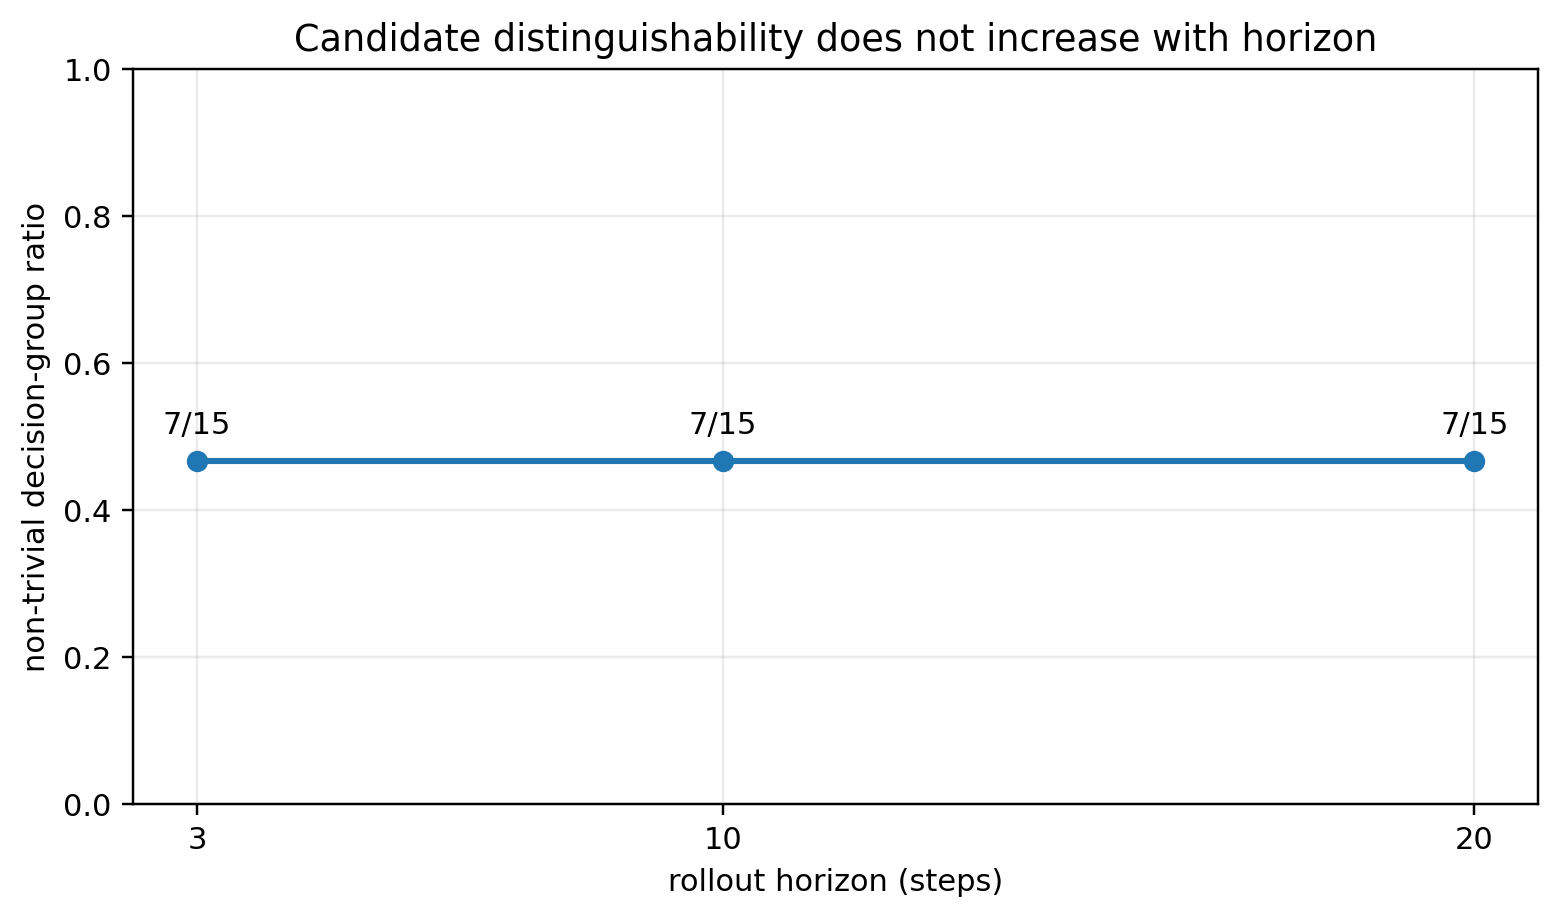
\includegraphics[width=0.88\linewidth]{figs/pi_jwm_horizon_nontrivial_ratio.png}
\caption{候选区分度随 rollout horizon 的变化。$H=3,10,20$ 均只有 7/15 个非平凡决策组，延长观察窗口没有增加有效排序监督。}
\label{fig:horizon_nontrivial_ratio_overview}
\end{figure}

\begin{figure}[H]
\centering
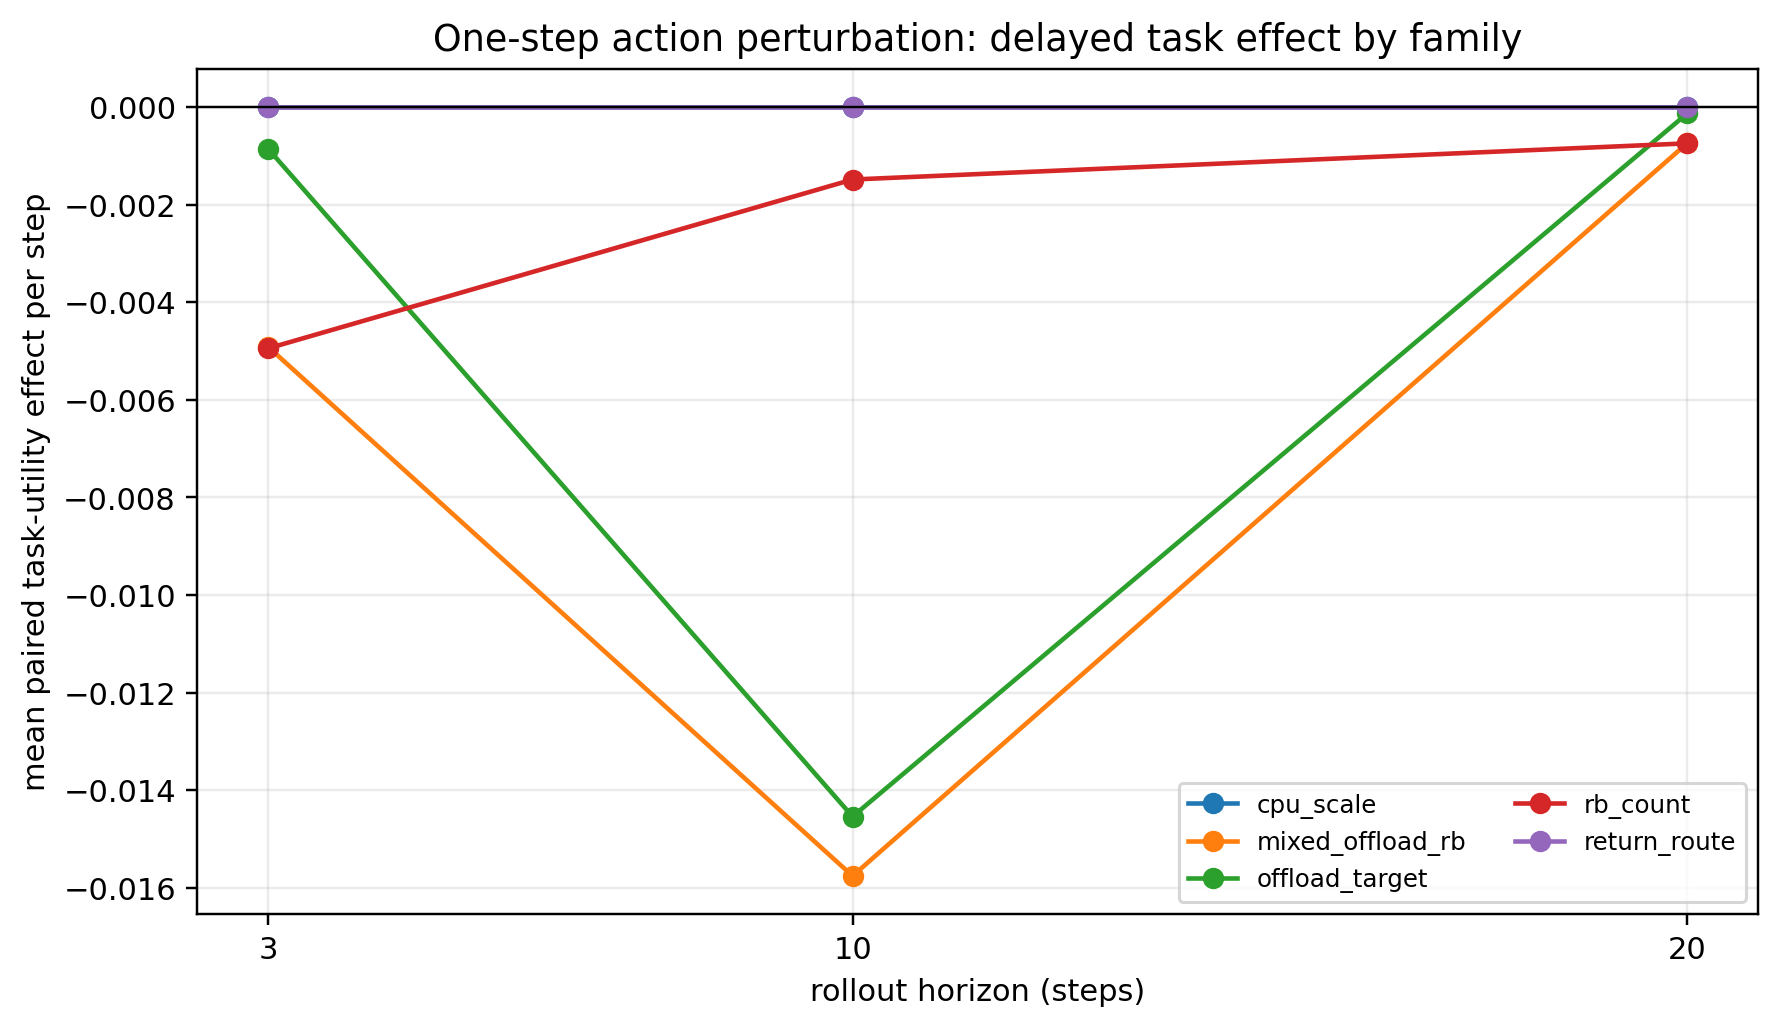
\includegraphics[width=0.92\linewidth]{figs/pi_jwm_horizon_family_task_effect_per_step.png}
\caption{单步动作扰动在不同 horizon 下的单位步 task-utility 配对效应。曲线表示动作族均值，只用于描述暂态效应，不表示跨 horizon 的策略性能排序。}
\label{fig:horizon_family_effect_overview}
\end{figure}

结果给出三个边界明确的判断。第一，$\rho_H$ 在三个 horizon 下均为 46.67\%，因此短窗口不是候选监督稀疏的唯一原因。第二，CPU-scale 的 12 个候选和 return-route 的 4 个候选在三个 horizon 下仍无可辨识效应；这不能推出 CPU/return 长期无效，只能说明当前决策点、动作幅度或一次性注入协议没有产生可测差异。第三，offload-target 与 mixed-offload-RB 在 $H=10$ 的单位步平均效应分别为 $-0.014543$ 和 $-0.015761$，到 $H=20$ 回到 $-0.000129$ 和 $-0.000737$，表现为中期负效应与后续补偿；该非单调变化不支持“horizon 越长越差”的结论。

能耗配对差异没有随 $H$ 累积，这是实验协议的直接结果：候选只改变第一步动作，后续调度相同。因而本轮能够支持的结论是，当前 actual-rollout candidate library 的有效监督覆盖不足，且部分 offload 效应具有暂态性；它不能证明某个 selector 或某个 $\lambda$ 已经改善策略。下一步应先构造持续多步候选序列、扩大 compute/return 有效决策点覆盖，再接入 PI-JWM forecast 与不确定性做 rollout-aware selector。完整数据、公式口径、复现命令和 SHA-256 冻结清单位于 \code{代码/artifacts/reports/pi\_jwm\_energy\_reward\_horizon\_study\_20260713/}。

\end{document}
